\documentclass{article}
\usepackage[utf8]{inputenc}
\usepackage[english]{babel}
\usepackage[]{amsthm} %lets us use \begin{proof}
\usepackage[]{amssymb} %gives us the character \varnothing
\usepackage{graphicx}
\usepackage{amsmath}
\usepackage{array}
\usepackage[a4paper]{geometry}


\begin{titlepage}
    \begin{center}
        \vspace*{1cm}
            
        \Huge
        \textbf{Trabajo Práctico 1}
            
        \vspace{0.5cm}
        \LARGE
        \textbf{Aprendizaje Estadístico}
            
        \vspace{1.5cm}
            
        Ignacio Brusati - Federico Elías
            
        \vfill
            
        \vspace{0.8cm}
            
            
    \end{center}
\end{titlepage}


\begin{document}







\section{Definición de variables}

En primer lugar se corrobora que todas las variables del dataset estén bien definidas. En este caso, dado que la variable 'Outcome' estaba definida como una variable continua entre 0 y 1, se la transformó en factor ya que representa dos categorías: la paciente tiene diabetes o la paciente no tiene diabetes. Por otra parte, se eliminó la variable 'X' que es simplemente un índice de las observaciones.





\section{Modelo de regresión múltiple para predecir la variable BMI en función del resto de las variables}

El modelo propuesto es:

$$Y = \beta_0 + \beta_1 x_1 + ... + \beta_{p-1} x_{p-1} + \epsilon$$\\

\noindent
donde \(x_i\) son las covariables, \(\beta_i\) son los parámetros a estimar, \(p\) es la cantidad de parámetros a estimar y \(\epsilon\)
 es el error aleatorio.\\

\noindent
Ajustado a los datos particulares de este problema, se desean estimar \(p = 9\) parámetros y el modelo tiene la forma:

$$BMI = \beta_0 \, + \, \beta_1 \, Pregnancies \, + \, \beta_2 \, Glucose \, + \, \beta_3 \, BloodPressure \, + \, \beta_4 \, SkinThickness \,
+ \, \beta_5 \, Insulin  \, + $$
$$\beta_6 \, DiabetesPedigreeFunction \, + \, \beta_7 \, Age \, + \, \beta_8 \, Outcome \, + \, \epsilon $$\\

\noindent
Los supuestos del modelo propuesto son:
\begin{itemize}
\item La media de los errores \(\epsilon_i\) es 0 para todos los errores.
\item La varianza de los errores \(\epsilon_i\) es \(\sigma^2\) para todos los errores.
\item Los errores \(\epsilon_i\) tienen distribución Normal, son independientes entre sí y no están correlacionados con las covariables \(X_i\).
\end{itemize}





\section{Scatterplots de las covariables}

\begin{center}
    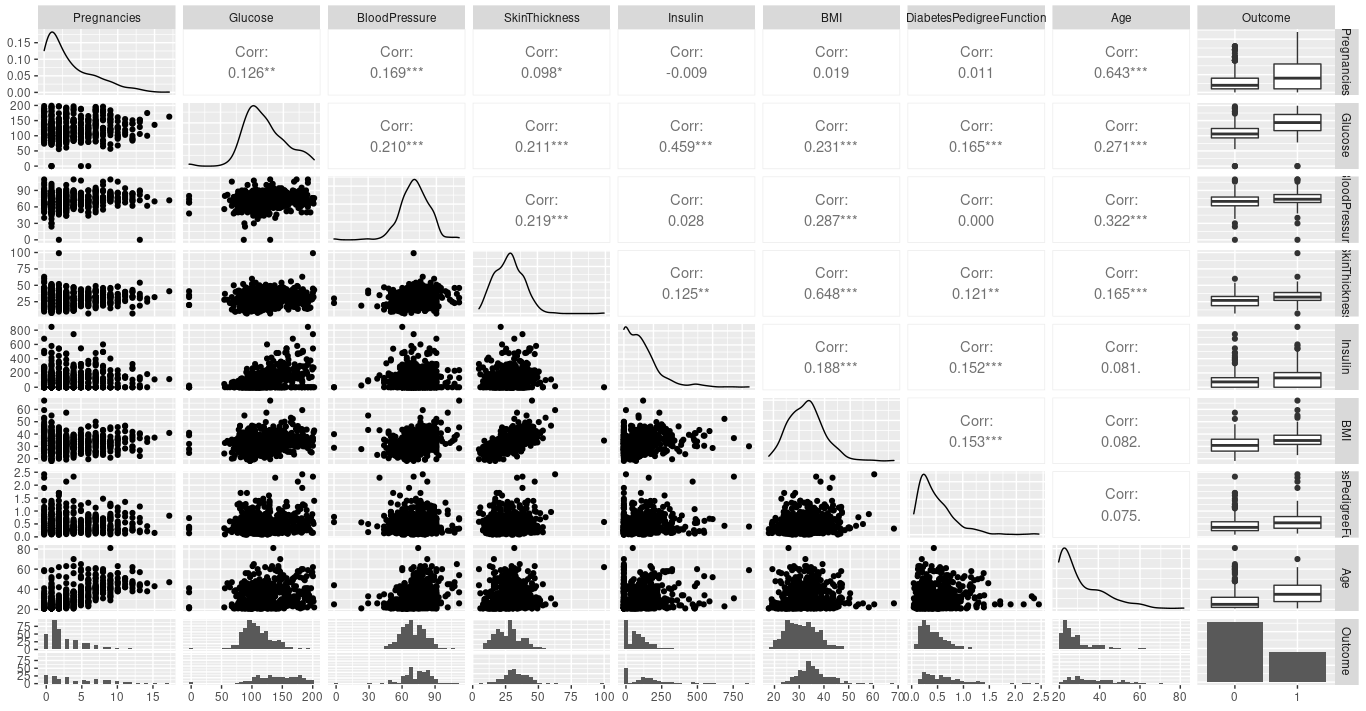
\includegraphics[width=1\textwidth]{img/scatterplot.png}
\end{center}

\noindent
Se observa que hay una alta correlación entre las covariables 'Glucose' e 'Insulin', y las covariables 'Age' y 'Pregnancies'. Por otro lado, la covariable 'Skin Thickness' es la que mayor correlación tiene con la variable 'BMI' que se desea predecir.\\

\noindent
Además, se observan valores de 0 para las covariables 'Glucose' y 'Blood Pressure'. Esto no tiene sentido médico y se asume que se debe a un error en el ingreso de los datos. Por lo tanto, esas muestras son eliminadas.\\

\noindent
Por otra parte, hay un claro outlier que se puede apreciar en la variable 'Skin Thickness'. Dado que ese outlier puede perjudicar las predicciones realizadas, se lo elimina de las muestras.\\

\noindent
A continuación se puede ver los nuevos scatterplots de las covariables:

\begin{center}
    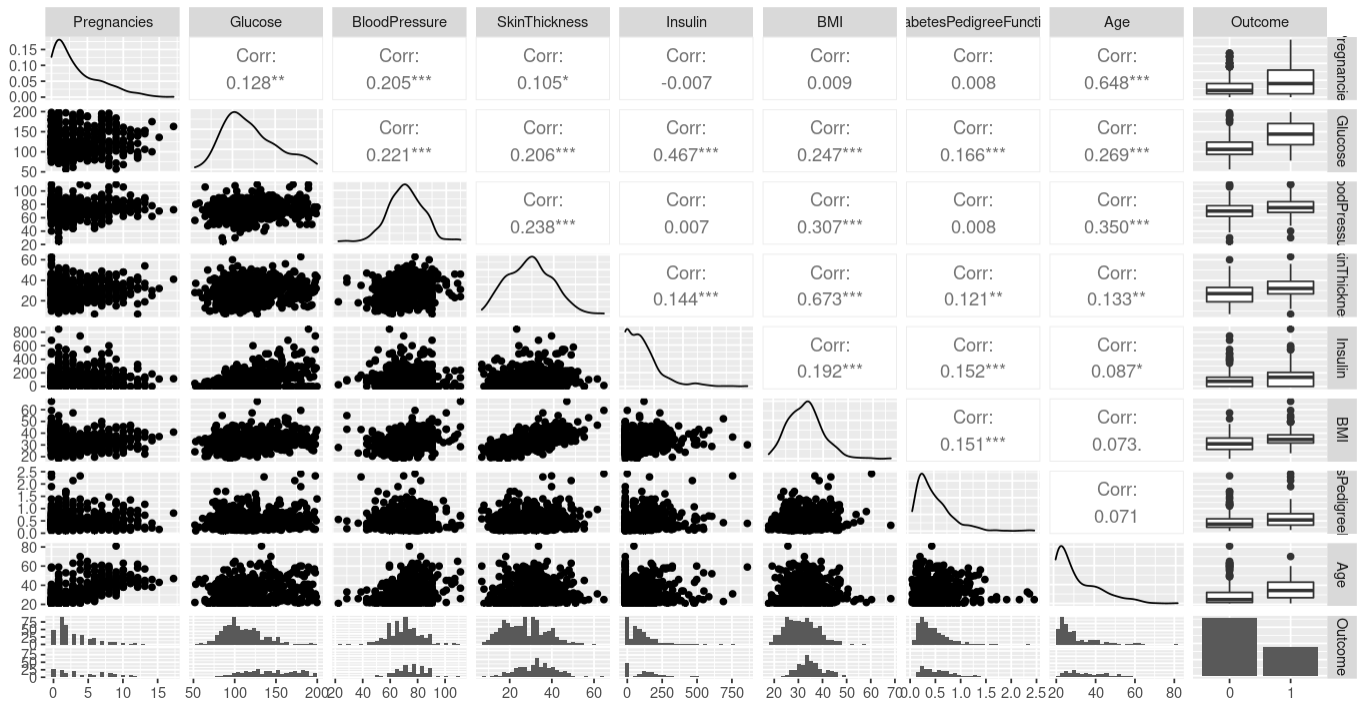
\includegraphics[width=1\textwidth]{img/scatterplot_sin_outliers.png}
\end{center}



\section{Elección de una sola variable en base a la tabla de correlaciones estimadas}

\noindent
A partir de la tabla de correlaciones estimadas entre las variables, si solo se tuviese que elegir una covariable lo mejor sería elegir a 'SkinThickness' ya que es la que mayor correlación tiene con la variable a predecir ‘BMI’. Es importante destacar que aunque 'SkinThickness' sea la covariable que mayor correlación tenga con la variable objetivo esto no impide que haya otras covariables que en conjunto resulten tener mayor correlación con la variable a predecir.





\section{Ajuste de regresión lineal múltiple}
Se realiza el ajuste de regresión lineal múltiple y se obtienen los coeficientes \(\beta_i\). Así, se puede escribir al modelo de la siguiente manera:

$$\widehat{BMI} = 14.174301 \, - \, 0.166560 \, Pregnancies \, + \, 0.001495 \, Glucose \, +$$
$$0.100203 \, BloodPressure \, + \, 0.408410 \, SkinThickness \, +$$
$$0.004028 \, Insulin  \, + 0.789812 \, DiabetesPedigreeFunction \, - \, 0.044974 \, Age \, +$$
$$1.949292 \, Outcome$$\\

\noindent
Por cada una de los parámetros \(\beta_i\) se realiza un test de hipótesis univariado para analizar si la covariable asociada a ese \(\beta_i\) resulta significativa. Asi, se plantean tests con la forma:

$$H_0: \beta_i = 0\qquad vs\qquad H_1: \beta_i \neq 0$$\\

\noindent
La regla de decisión del test entonces resulta:

$$\varphi(\underline{X}) = \begin{cases}
                            1 \; \; \text{si} \; \;  |T| > k_{\alpha}\\
                            0 \; \; \text{en otro caso}
                        \end{cases}$$

\noindent
El estadístico del test es:

$$T = \frac{\hat{\beta_i}}{S \sqrt{d_{ii}}}$$\\

\noindent
siendo \(d_{ii}\) el elemento i de la diagonal de la matriz \(D = (X^T X)^{-1}\) y \(S^2\) un estimador de la varianza de Y. Además, se sabe que el estadístico bajo \(H_0\) tiene distribución t-Student con \(n - p\) grados de libertad.\\

\noindent
El valor de \(k_\alpha\) surge de:

$$\alpha = P_{H_0}(\varphi(\underline{X})=1)$$\\

\noindent
El \(p-valor\) en este caso se calcula como:

$$\text{p-valor} = 2 P(T > |t_{obs}|)$$\\

\noindent
En el caso particular del modelo propuesto, se realizó para todos los parámetros un test de hipótesis univariado de nivel 0.05. Por lo tanto si \(p-valor < 0.05\) entonces se rechaza la hipótesis nula y se confirma la alternativa. En otras palabras, si \(p-valor < 0.05\) entonces se puede asegurar que la variable resulta significativa. En el modelo propuesto, las variables que resultan significativas a nivel de significación 0.05 son:

\begin{itemize}
\item BloodPressure
\item SkinThickness
\item Insulin
\item Pregnancies
\item Outcome
\end{itemize}

\noindent
Finalmente, el valor de la estimación para \(\sigma^2\) es 23.44496.





\section{Coeficiente de determinación}

El coeficiente de determinación \(R^2\) mide el porcentaje de la variabilidad de Y explicado por el modelo de regresión propuesto y se define como:

$$R^2 = \frac{||\hat{Y} - \overline{Y}||^2}{||Y - \overline{Y}||^2}$$

\noindent
El valor de \(R^2\) toma valores entre 0 y 1, y mientras más cerca está de 1, mejor se explica la variabilidad de Y respecto a las otras variables. Sin embargo, a medida que se aumenta la cantidad de covariables el valor del coeficiente de determinación va a aumentar sin importar si realemente esa covariable agregada está aportando información. Es por esto que la fórmula del coeficiente de determinación necesita un ajuste cuando hay varias covariables que penalice el agregado de nuevas covariables para asegurar que el coeficiente aumenta si realmente esa covariable agregada es significativa. Así, se define al coeficiente de determinación ajustado:

$$R_a^2 = 1- \frac{||Y - \hat{Y}||^2}{||Y - \overline{Y}||^2} \frac{n - 1}{n - p}$$\\

\noindent
En el caso particular del modelo propuesto, el coeficiente de determinación ajustado es 0.5058.\\

\noindent
A partir de este coeficiente se deduce que las covariables observadas son importantes para predecir a la variable objetivo pero que posiblemente haya una o varias variables que no fueron observadas y que puedan contribuir a explicar a la variable objetivo.





\section{Test de significación de la regresión}

\noindent
Para que la regresión sea significativa por lo menos algún \(\beta_i\) debe ser diferente de 0. De no cumplirse esta condición, la regresión perderá su utilidad para este caso y convendría utilizar al promedio para estimar la esperanza de Y.\\

\noindent
Para poder comprobar si la regresión es significativa se plantea el siguiente test de hipótesis:

$$H_0: \beta_1 = ... = \beta_8 = 0\qquad vs\qquad H_1: \text{algún}\, \beta_i \neq 0$$

\noindent
Se puede reescribir el test matricialmente de la siguiente manera:

$$H_0: C\, \beta = \delta \qquad vs\qquad H_1: C\, \beta \neq \delta$$

\noindent
Las matrices utilizadas para el test en el caso puntual del modelo propuesto son:\\

$$
C = \begin{pmatrix}
0 & 1 & 0 & 0 & 0 & 0 & 0 & 0 & 0\\
0 & 0 & 1 & 0 & 0 & 0 & 0 & 0 & 0\\
0 & 0 & 0 & 1 & 0 & 0 & 0 & 0 & 0\\
0 & 0 & 0 & 0 & 1 & 0 & 0 & 0 & 0\\
0 & 0 & 0 & 0 & 0 & 1 & 0 & 0 & 0\\
0 & 0 & 0 & 0 & 0 & 0 & 1 & 0 & 0\\
0 & 0 & 0 & 0 & 0 & 0 & 0 & 1 & 0\\
0 & 0 & 0 & 0 & 0 & 0 & 0 & 0 & 1
\end{pmatrix}
$$

$$
\beta = \begin{pmatrix}
\beta_0\\
\beta_1\\
\beta_2\\
\beta_3\\
\beta_4\\
\beta_5\\
\beta_6\\
\beta_7\\
\beta_8
\end{pmatrix}
\qquad  \qquad
\delta = \begin{pmatrix}
0\\
0\\
0\\
0\\
0\\
0\\
0\\
0
\end{pmatrix}
$$\\

\noindent
con \(p=9\) y \(n=531\).\\

\noindent
La regla de decisión del test entonces resulta:

$$\varphi(\underline{X}) = \begin{cases}
                            1 \; \; \text{si} \; \;  F > \mathcal{F}_{p-1,n-p,1-\alpha}\\
                            0 \; \; \text{en otro caso}
                        \end{cases}$$

\noindent
El estadístico del test es:

$$F = \frac{(C\hat{\beta}-\delta)^T(C(X^TX)^{-1})C^T)^{-1}(C\hat{\beta}-\delta)}{(p-1)S^2}$$\\

\noindent
Se sabe que el estadístico bajo \(H_0\) tiene distribución de Fischer de parámetros \(p-1\) y \(n - p\).\\

\noindent
El valor de \(\mathcal{F}_{p-1,n-p,1-\alpha}\) surge de:

$$\alpha = P_{H_0}(\varphi(\underline{X})=1)$$\\

\noindent
El \(p-valor\) en este caso se calcula como:

$$\text{p-valor} = P(F \geq f_{obs})$$\\

\noindent
En el caso particular del modelo propuesto, se realizó el test de significación de la regresión con nivel 0.95. Como \(p-valor < 0.05\) entonces se rechazó la hipótesis nula y se confirmó la alternativa. De esta forma, se confirmó que la regresión es significativa.\\

\noindent
A un nivel de significación de 0.05 rechazaría la hipótesis nula ya que es el límite que generalmente se utiliza para estos tests.





\section{Estimación de la esperanza del BMI para una nueva observación independiente}

Si llegara una nueva observación con los siguientes datos:
\begin{itemize}
  \item Embarazos: 2
  \item Concentración de glucosa: 100
  \item Presión sistólica: 70
  \item Valor de piel de tríceps: 20
  \item Función pedigree: 0.24
  \item Edad: 30
  \item Diabetes: no
\end{itemize}

\noindent
se debe observar que no se posee una medición para la variable 'Insulin'. De esta forma, el modelo que se venía utilizando no puede ser usado en este caso. Se debe entonces generar un nuevo modelo sin la variable 'Insulin':

$$BMI = \beta_0 \, + \, \beta_1 \, Pregnancies \, + \, \beta_2 \, Glucose \, + \, \beta_3 \, BloodPressure \, + \, \beta_4 \, SkinThickness \, + $$
$$\beta_5 \, DiabetesPedigreeFunction \, + \, \beta_6 \, Age \, + \, \beta_7 \, Outcome \, + \, \epsilon $$\\

\noindent 
De esta forma se tiene un parámetro menos a predecir y por lo tanto \(p = 8 \).\\

\noindent
Con el nuevo modelo, la esperanza estimada del BMI de una mujer que cumple con los datos indicados será de 28.28866.







\section{Intervalos de confianza y de predicción}
\textbf{Intervalo de confianza de nivel 0.95 para la estimación hallada en el ıtem anterior}\\

\noindent
Según el modelo se sabe que \(Y|\underline{X}=\underline{x}\) tiene distribución \(N_n(X \beta, \sigma^2 I)\). Por lo tanto \(E(Y_i|\underline{X}=\underline{x_i}) = x_i^T \beta\).\\

\noindent
Se desea encontrar un intervalo de confianza para la esperanza de una nueva observación independiente \((y_0, \underline{x_0})\) donde \(\underline{x_0}\) son los nuevos datos e \(y_0\) es lo que se desea predecir. Es decir, se quiere predecir \(E(Y_0|\underline{X}=x_0) = x_0^T \beta\).\\

\noindent
La estimación de \(E(Y_0|\underline{X}=x_0) = x_0^T \beta\) es \(\widehat{E(Y_0|\underline{X}=x_0)} = x_0^T \hat{\beta} = \hat{y_0}\) cuya distribución es \(N(x_0^T \beta, \sigma ^2 x_0^T (X^T X)^{-1}x_0))\)\\

\noindent
Un pivote para este caso es:\\

$$T = \frac{\hat{Y_0} - x_0^T \beta}{S \sqrt{x_0^T (X^T X)^{-1} x_0}}$$\\

\noindent
el cual tiene distribución t-Student con \(n-p\) grados de libertad.\\

\noindent
De esta forma, el intervalo de confianza de nivel \(1-\alpha\) es:

$$IC = [\hat{y_0} \ - \ t_{n-p, 1-\frac{\alpha}{2}} \ S \ \sqrt{x_0^T \ (X^T \ X)^{-1} \ x_0} \ ; \ \hat{y_0} \ + \ t_{n-p, 1-\frac{\alpha}{2}} \ S \ \sqrt{x_0^T \ (X^T \ X)^{-1} \ x_0}]$$\\

\noindent
Para el caso particular en el que \(\hat{y_0} \ = \ 28.28866\), la cantidad de observaciones \(n \ = \ 531\), la cantidad de parámetros a estimar \(p \ = \ 8\) y \(\alpha \ = \ 0.05\)\\

$$x_0 = (1, 2, 100, 70, 20, 0.24, 30, 0)$$

$$
X = \begin{pmatrix}
1 & x_{1,1} & ... & x_{1,p-1}\\
1 & x_{2,1} & ... & x_{2,p-1}\\
. & . & . & .\\
. & . & . & .\\
. & . & . & .\\
1 & x_{n,1} & ... & x_{n,p-1}
\end{pmatrix}
$$\\

\noindent
el intervalo de confianza es:

$$IC = [27.60400; 28.97332]$$\\

\noindent
\textbf{Intervalo de predicción de nivel 0.95 para la estimación hallada en el ıtem anterior}\\

$$IC = [\hat{y_0} \ - \ t_{n-p, 1-\frac{\alpha}{2}} \ S \ \sqrt{1 + x_0^T \ (X^T \ X)^{-1} \ x_0} \ ; \ \hat{y_0} \ + \ t_{n-p, 1-\frac{\alpha}{2}} \ S \ \sqrt{1 + x_0^T \ (X^T \ X)^{-1} \ x_0}]$$\\

\noindent
Para el caso particular en el que \(\hat{y_0} \ = \ 28.28866\), la cantidad de observaciones \(n \ = \ 531\), la cantidad de parámetros a estimar \(p \ = \ 8\) y \(\alpha \ = \ 0.05\)\\

$$x_0 = (1, 2, 100, 70, 20, 0.24, 30, 0)$$

$$
X = \begin{pmatrix}
1 & x_{1,1} & ... & x_{1,p-1}\\
1 & x_{2,1} & ... & x_{2,p-1}\\
. & . & . & .\\
. & . & . & .\\
. & . & . & .\\
1 & x_{n,1} & ... & x_{n,p-1}
\end{pmatrix}
$$\\

\noindent
el intervalo de predicción es:

$$IP = [18.72367; 37.85364]$$\\





\section{Selección de modelos}

\noindent
Para realizar la selección del menor subconjunto de covariables que optimicen el modelo final se utilizó el método Best Subset el cual estudia las \(2^{p-1}\) regresiones posibles y se termina eligiendo la que tenga el menor error cuadrático medio.\\

\noindent
En el caso del modelo propuesto se evaluaron las \(2^{8}\) regresiones y para cada una de ellas se calculó una estimación del error cuadrático medio usando Cross Validation:\\

$$\widehat{ECM} = \frac{1}{n} \sum_{i=1}^{n} \frac{r^2}{(1 - p_{ii})^2}$$\\

\noindent
El modelo que resultó tener el menor error cuadrático medio es:\\

$$BMI = \beta_0 \, + \, \beta_1 \, BloodPressure \, + \, \beta_2 \, SkinThickness \,
+ \, \beta_3 \, Pregnancies \, + \, \beta_4 \, Outcome \, + \, \epsilon $$\\

\noindent
con un error de \(25.18543\) usando una semilla de \(13\).\\

\noindent
El modelo completo con sus coeficientes es:

$$BMI = 14.56481 \, + \, 0.08964 \, BloodPressure \, + \, 0.41664 \, SkinThickness \,
- $$
$$0.26380 \, Pregnancies \, + \, 2.22374 \, Outcome \, + \, \epsilon $$\\

\noindent
Algo importante a destacar es que este modelo tiene un coeficiente de determinación (\(0.5007\)) algo menor que el modelo que había sido propuesto al principio pero con la diferencia de que este modelo tiene 3 covariables menos. Esto significará seguramente ahorro en esfuerzos de medición de esas variables y además se obtiene un modelo más sencillo de explicar.\\

\noindent
Se destaca que las variables eliminadas son 'Age', 'Insulin', 'Glucose' y 'DiabetesPedigreeFunction'. Este resultado tiene sentido ya que en la tabla de correlaciones se había observado que la variable 'Glucose' tenía una alta correlación con la variable 'Insulin'. Lo mismo sucedía con la variable 'Pregnancies' que tenía una alta correlación con la variable 'Age'. En el modelo final entonces se asegura que no queden covariables correlacionadas entre sí. Además, se puede observar que todas las covariables que quedan en el modelo final resultaron significativas al realizar el test de hipótesis en la sección 1.5, lo cual es positivo. De las 4 covariables que fueron eliminadas del modelo, 3 de ellas ('Glucose', 'Age', y 'DiabetesPedigreeFunction') en sus respectivos tests de hipótesis no se pudo rechazar la hipótesis nula y por lo tanto no se pudo asegurar que fueran significativas. De esta manera, se obtiene un modelo final con covariables significativas y poco correlacionadas entre sí.





\section{Validación de supuestos}
\textbf{Supuesto 1: La media de los errores \(\epsilon_i\) es 0 para todos los errores}\\

\noindent
Para validar este supuesto se calcula la media de los residuos. En este caso la media de los residuos dio \(0.000421385\) lo cual es un valor muy cercano a 0 y por lo tanto queda validado este supuesto.\\


\noindent
\textbf{Supuesto 2: La varianza de los errores \(\epsilon_i\) es \(\sigma^2\) para todos los errores}\\

\noindent
Para validar este supuesto se realiza un gráfico de la distribución de los residuos estandarizados en función de los valores ajustados por el modelo:\\

\begin{center}
    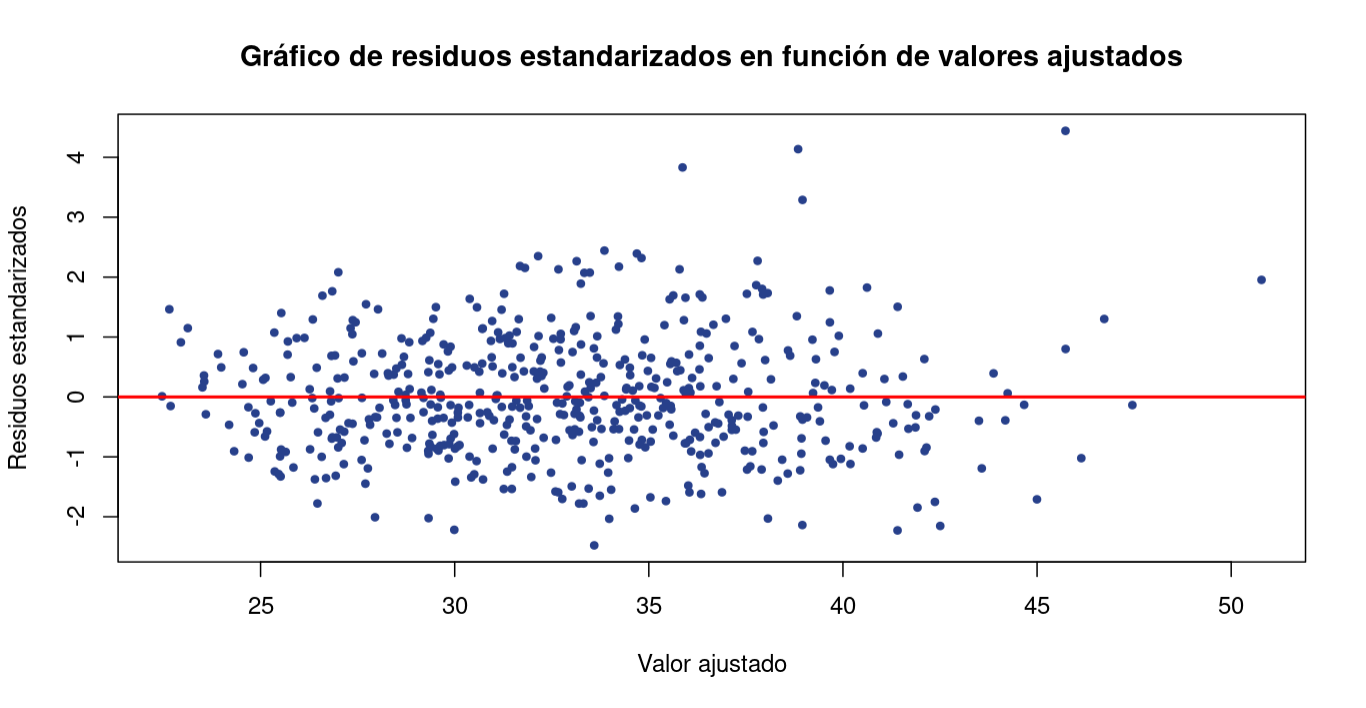
\includegraphics[width=1\textwidth]{img/residuos.png}
\end{center}

\noindent
Se puede observar que los residuos forman una nube de puntos heterogénea alrededor del 0 sin formar ningún tipo de patrón. De esta forma, se puede corroborar la hipótesis 2.\\

\noindent
\textbf{Supuesto 3: Los errores \(\epsilon_i\) tienen distribución Normal.}\\

\begin{center}
    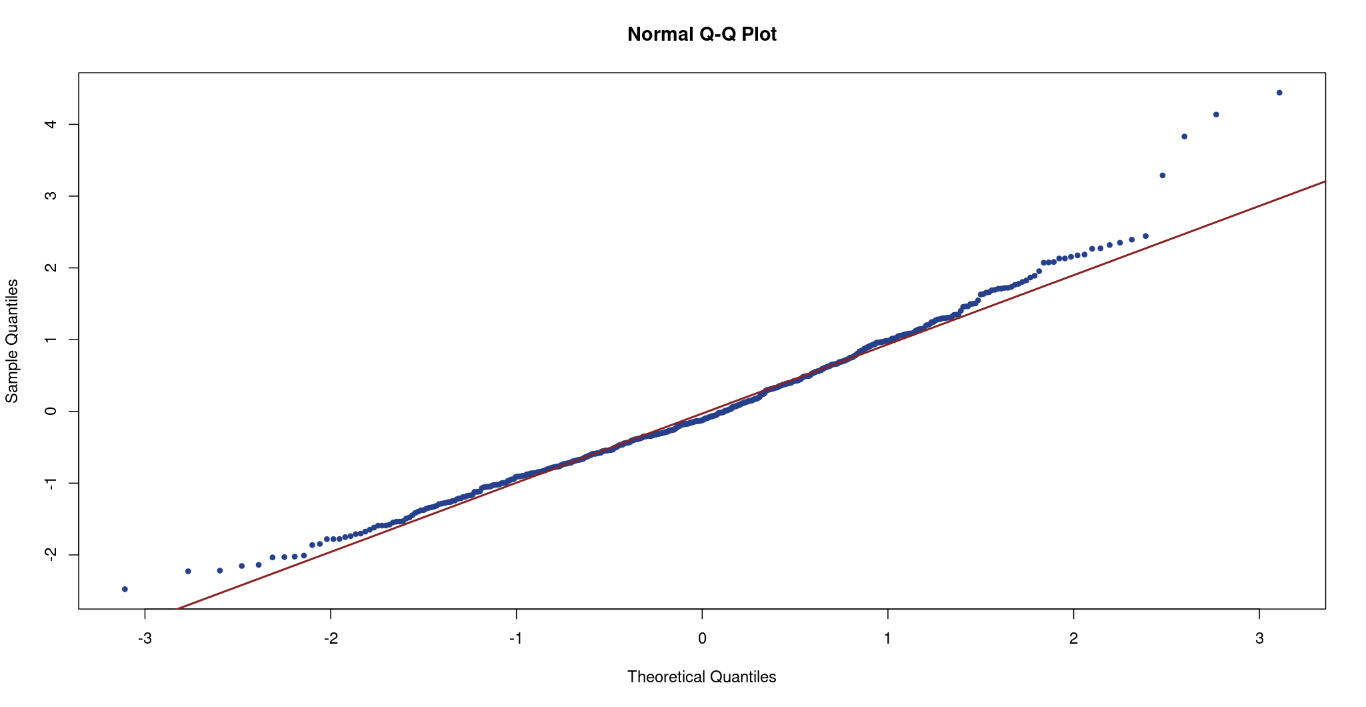
\includegraphics[width=1\textwidth]{img/qqplot.png}
\end{center}

\noindent
Se observa que los errores parecerían tener distribución normal pero tienen colas pesadas. De esta forma se realiza una transformación Box-Cox dada por:

$$y^{(\lambda)} = \begin{cases}
                            \frac{y^{\lambda}-1}{\lambda} \; \; \text{si} \; \;  \lambda \neq 0\\
                            log(\lambda) \; \; \text{si} \; \; \lambda = 0
                        \end{cases}$$

\noindent
A continuación se puede ver un gráfico de los diferentes $\lambda$ probados y sus verosimilitudes:

\begin{center}
    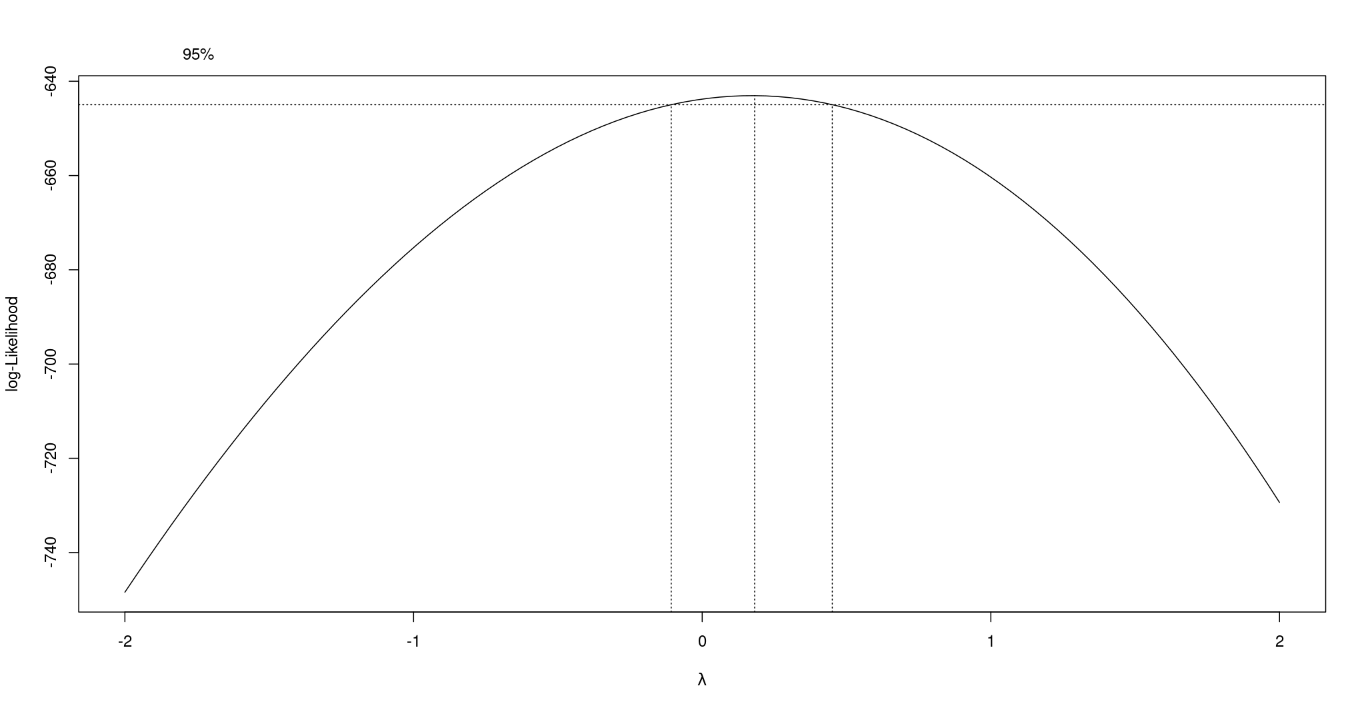
\includegraphics[width=1\textwidth]{img/lambdas.png}
\end{center}

\noindent
El $\lambda$ que maximiza la verosimilitud es 0.1818182.\\

\noindent
Luego de realizar la transformación entonces se vuelven a validar los supuestos. La media de los residuos dio \(0.0002814912\) lo cual es un valor muy cercano a 0 y por lo tanto queda validado este supuesto. Además, se puede observar a continuación que los residuos forman una nube de puntos heterogénea alrededor del 0 sin formar ningún tipo de patrón. De esta forma, se puede corroborar la hipótesis 2.

\begin{center}
    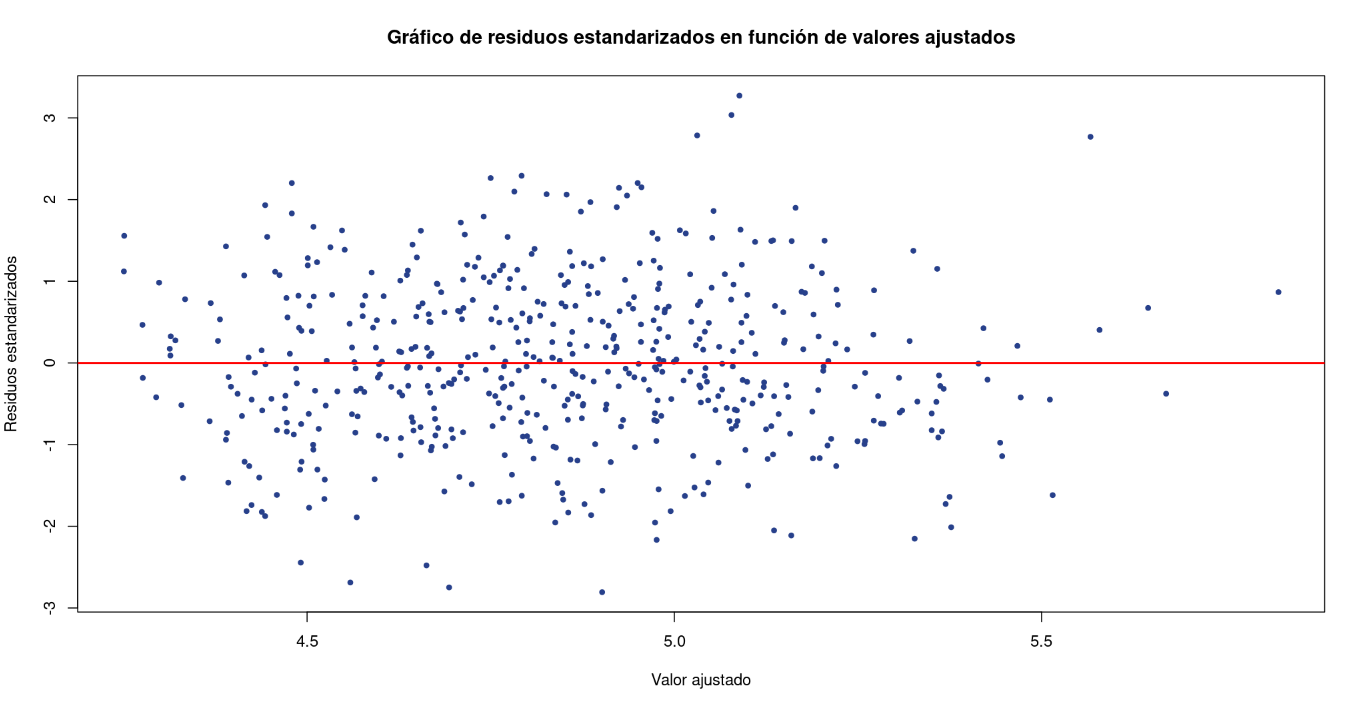
\includegraphics[width=1\textwidth]{img/bc_residuos.png}
\end{center}

\noindent
Finalmente, se observa que los errores tienen distribución normal y desaparecieron las colas pesadas:

\begin{center}
    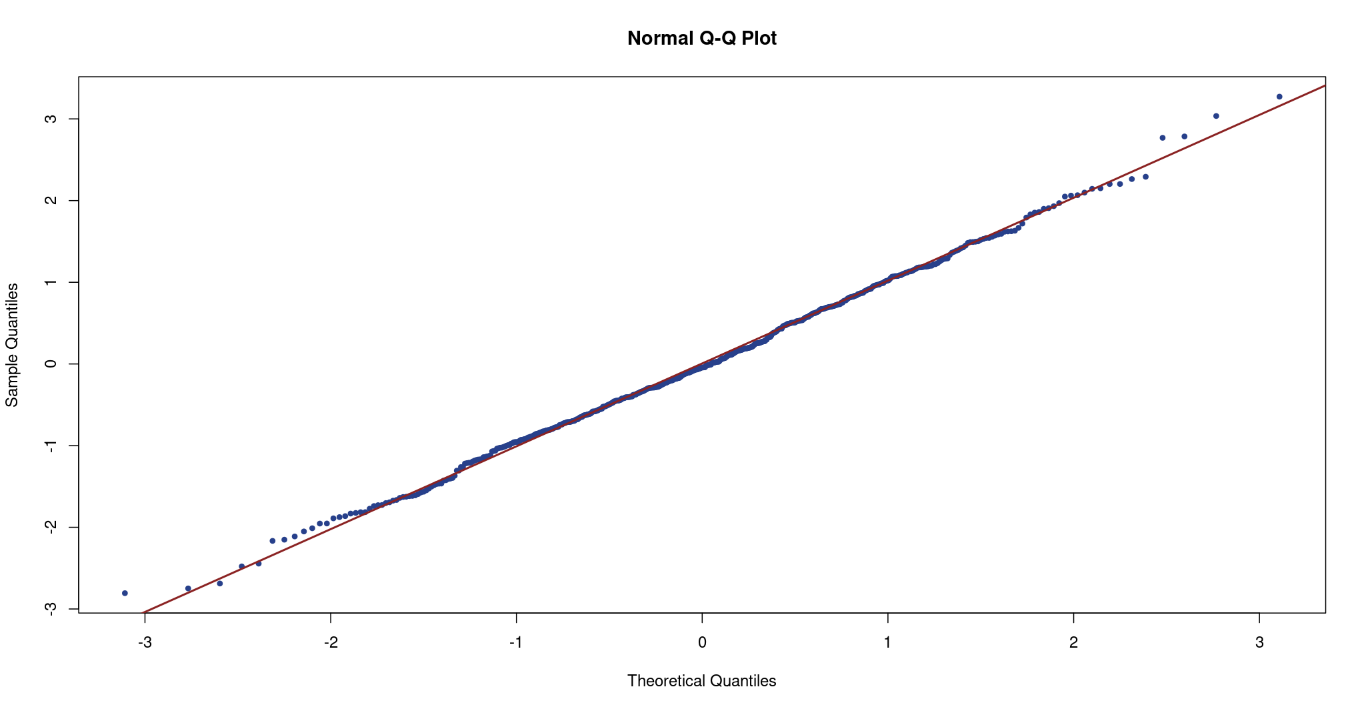
\includegraphics[width=1\textwidth]{img/bc_qqplot.png}
\end{center}

\noindent
El modelo completo con sus coeficientes luego de realizar la transformación es:

$$BMI = 3.811446 \, + \, 0.004752 \, BloodPressure \, + \, 0.023999 \, SkinThickness \,
- $$
$$0.012662 \, Pregnancies \, + \, 0.128494 \, Outcome \, + \, \epsilon $$


\section{Estimación de la densidad del estimador del coeficiente de regresión de 'SkinThickness' mediante bootstrap no paramétrico}

\noindent
Para estimar la densidad del estimador del coeficiente de regresión de 'SkinThickness' mediante bootstrap no paramétrico primero se generaron 1000 muestras de tamaño $n=539$, realizando extracciones con reposición de la muestra original. Luego, para cada una de las muestras generadas se encontró una estimación del coeficiente de regresión.\\

\noindent
Finalmente se realizó un histograma para poder observar la distribución del estimador:\\

\begin{center}
    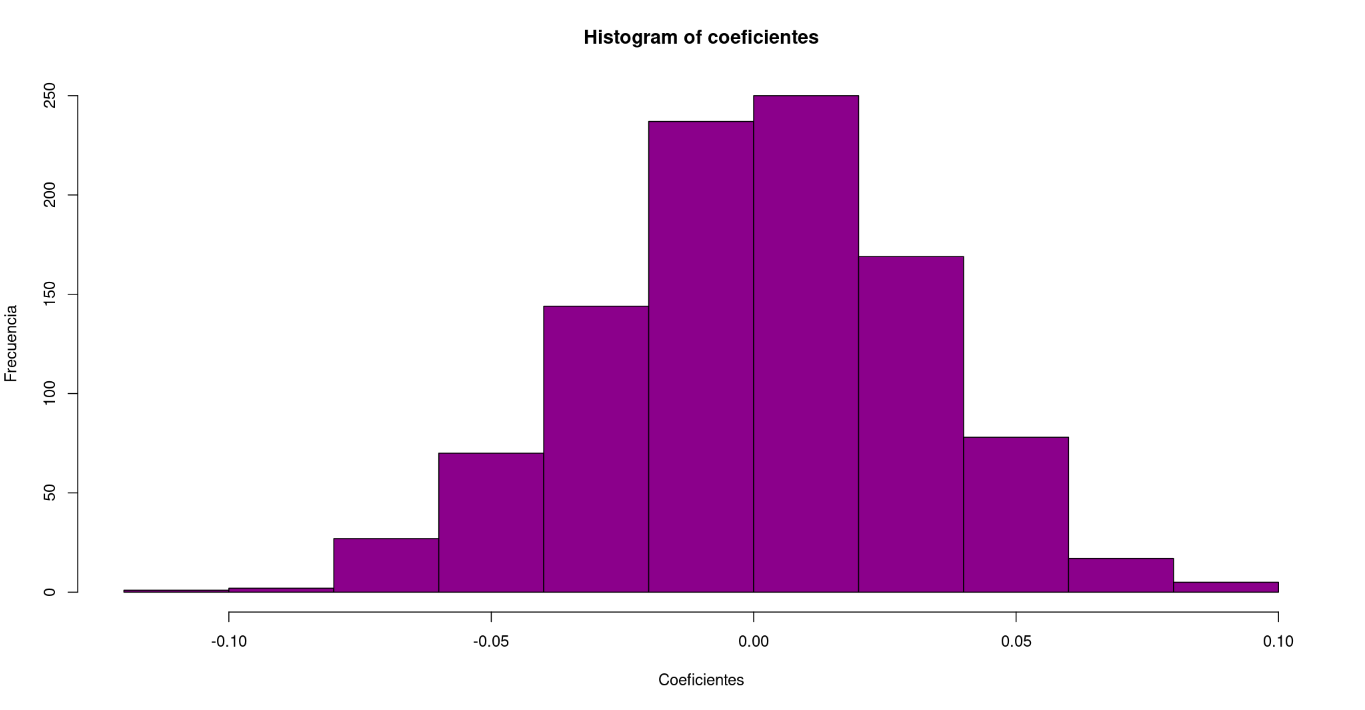
\includegraphics[width=1\textwidth]{img/histograma.png}
\end{center}

\noindent
Se puede observar que el estimador tiene una distribución acampanada con media en el 0. Esto último es llamativo ya que el coeficiente de regresión que fue utilizado en el modelo final fue 0.380439. Es probable entonces que la covariable 'SkinThickness' esté correlacionada con el resto de las covariables y por lo tanto al tomar nuevas muestras y calcular nuevamente los coeficientes de regresión, estos ya hayan perdido esa relación y por lo tanto el coeficiente deja de ser significativo.




\end{document}